

TODO: NACH TODO SUCHEN!!!!!!!!!!!!!!!!!!!!!!!!!!!!!!!!!!!!!!!!!!!!!!!!!!!!!!!!

!!!!!!!!!!!!!!!!!!!!!!!!!!!!!!!

!!!!!!!!!!!!!!!!!!!!!!!!!!!!!!!

!!!!!!!!!!!!!!!!!!!!!!!!!!!!!!!

!!!!!!!!!!!!!!!!!!!!!!!!!!!!!!!

!!!!!!!!!!!!!!!!!!!!!!!!!!!!!!!\\

!!!!!!!!!!!!!!!!!!!!!!!!!!!!!!!

!!!!!!!!!!!!!!!!!!!!!!!!!!!!!!!

!!!!!!!!!!!!!!!!!!!!!!!!!!!!!!!

!!!!!!!!!!!!!!!!!!!!!!!!!!!!!!!






\section{Technische Hintergründe}

\subsection{Geschichte des Ext-Dateisystems}

% TODO: hier bissl mehr?
% TODO: RE-READ ALLES FREITAG!!!!!!!!!!!!!!!
% TODO: AUCH GLEICH BLOG POST! mit paar screenshots vielleicht?

Das sogenannte \ac{ext} war das Erste einer Reihe von Dateisystemen welches speziell für Linux entwickelt wurde und damals das minix-Dateisystem ablöste. \ac{ext} in Version 1 ist mittlerweile allerdings veraltet und wird in aktuellen Linux-Distributionen nicht mehr verwendet. Ext3 ist die neuere Variante, bleibt von Grund auf jedoch exakt gleich wie Ext2, führt jedoch "file system journaling" ein. Die folgenden Varianten sind aktuell noch gängig und werden aktiv eingesetzt:

\begin{itemize}
	\item ext2 - Führte separate Zeitstempel für Dateizugriffe, Inode- und Datenmodifikation ein. Bringt keine Unterstützung für journaling.
	\item ext3 - Führte journaling ein (und ist required!)
	\item ext4 - Unterstützung für fast fsck, native filesystem encryption, journaling, jedoch auch für non-journaling
\end{itemize}


\subsection{Basics}

Das Ext-Dateisystem verwendet Blöcke als Basiseinheit zum Speichern von Daten \cite{Ext2.07.01.2022}. Sogenannte "Inodes (Index-Nodes) werden zum Speichern von Metadaten verwendet, Blockgruppen zur optimierten logischen Strukturierung, Verzeichnisse um hierarchische Strukturen darstellen zu können, Block- und Inode-Bitmaps um allokierte Blöcke und Inodes zu kennzeichnen, sowie Superblöcke um allgemeine Informationen des Dateisystems zu speichern. Kopien von wichtigen Datenstrukturen wie z.B. den Superblöcken werden redundant vorgehalten und alle Daten welche mit Dateien assoziiert werden, sind aus Gründen der Performance gut lokalisiert\cite{Carrier.06.01.2022}.

\begin{figure}[H]
	\centering
	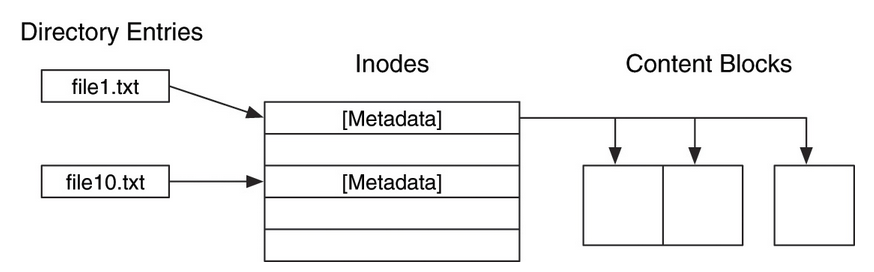
\includegraphics[width=12cm,keepaspectratio=true]{pictures/ext1.png}
	\caption{
		Zusammenhang zwischen Verzeichniseinträgen, Inodes und Inhaltsblöcken \cite{Carrier.06.01.2022}
	}
	\label{fig:ext1}
\end{figure}

Abbildung \ref{fig:ext1} zeigt den Zusammenhang zwischen Verzeichniseinträgen, Inodes und Inhaltsblöcken. Für jede Datei (und für jedes Verzeichnis) existiert eine Inode, welche dazugehörige Metadaten, sowie Referenzen auf die Blöcke mit dem tatsächlichen Inhalt speichert.

\begin{figure}[H]
	\centering
	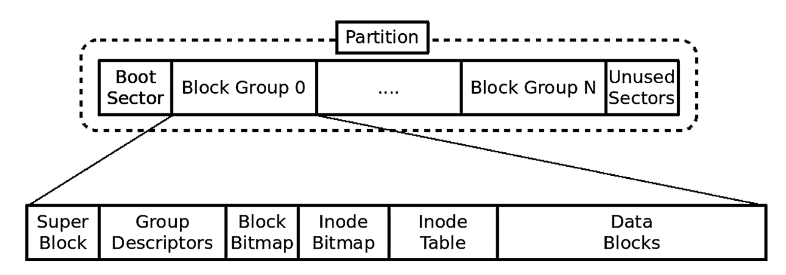
\includegraphics[width=12cm,keepaspectratio=true]{pictures/layout.png}
	\caption{
		Layout des Dateisystems \cite{AnalysisExt4.07.01.2022}
	}
	\label{fig:layout}
\end{figure}

Abbildung \ref{fig:layout} enthält eine graphische Darstellung des Layouts eines Ext-Dateisystems. Die Partition ist in Blockgruppen aufgeteilt und jede Blockgruppe enthält einen Superblock (optional), Group-Descriptors, die Block- und Inode-Bitmap, die Inode-Tabelle sowie die Datenblöcke. Auf diese Aufteilung innerhalb der Blockgruppen wird nun in den folgenden Unterkapiteln näher eingegangen.

\subsubsection{Superblöcke}

Da wir hier ein Ext3 System uf einem USB Stick erstellt haben und dieser keinen OS Kernel enthält, befindet sich auf unerem Stick auch kein Boot-Code. Dieser würde sich sonst in den ersten 1024 Bytes einer Platte befinden. Der \textit{Superblock} befindet sich ab Offset 1024 des Dateisystems und hat eine Größe von 1024 Bytes, obwohl nicht alle davon verwendet werden. Er enthält Basisinformation wie die Blockgröße, die totale Anzahl an Blöcken, die Anzahl an Blöcken pro Gruppe, die Anzahl an Inodes per Blockgruppe, den Volume-Name, den letzten Schreibzugriff, die letzte Mountzeit sowie den Pfad in dem das Dateisystem zuletzt gemounted war. Abbildung \ref{fig:superblock} zeigt eine simple Analyse des Superblocks auf unserem USB Stick.

\begin{figure}[H]
	\centering
	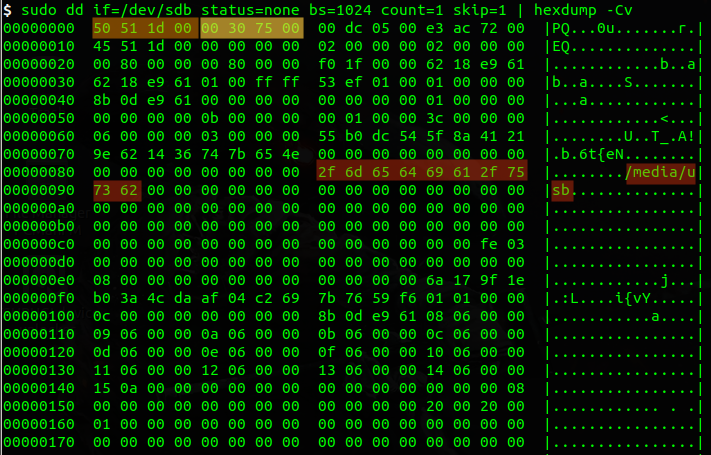
\includegraphics[width=12cm,keepaspectratio=true]{pictures/superblock.png}
	\caption{
		Analyse des Superblocks
	}
	\label{fig:superblock}
\end{figure}

Die ersten 4 Bytes repräsentieren die Anzahl an Inodes: \cite{Ext2.07.01.2022}:

\textbf{50 51 1d 00 -> Little endian -> 00 1D 51 50 ergibt 1921360 Inodes}(Vergleiche mit Abbildung \ref{fig:createfs}).\\Die zweiten 4 Bytes repräsentieren die Anzahl an Blöcken:

\textbf{00 30 75 00 => Little endien => 00 75 30 00 = ergibt 7680000 Blöcke}. Die Abbildung markiert außerdem noch den Pfad in welchem das Dateisystem zletzt gemounted war: \textbf{/media/usb}.


\subsubsection{Block Group Descriptor Tables}
Im Block nach dem Superblock folgt die Group-Descriptor-Tabelle. Diese beschreibt wo sich Daten wie z.B. die Inode-Tabelle oder die Bitmaps innerhalb einer Blockgruppe befinden. 


\subsubsection{Block- und Inode-Bitmaps}
Die Block- und Inode-Bitmaps speichern den Allokationsstatus von Blöcken, sowie Inodes innerhalb der Blockgruppe. Sie geben also an welche Blöcke- bzw Inodes innerhalb der Gruppe belegt sind und welche nicht. Jedes Bit repräsentiert hier den Status eines Blocks wobei "1" bedeutet, der Block ist verwendet, "0" bedeutet der Block ist frei bzw. verfügbar.

Die Inode-Bitmap funktioniert ähnlich, mit dem Unterschied dass die Bits hier auf den Allokationsstatus einer Inode-Tabelle verweisen.

\subsubsection{Die Inode-Tabelle}

Die Inode-Tabelle wird verwendet um jedes Verzeichnis, jede Datei, symbolischen Link oder Spezialdatei zu beschreiben. Die folgenden Metadaten werden u.a. in den Inodes gespeichert:

\begin{itemize}
	\item Dateigröße
	\item Speicherort
	\item Eigentümer
	\item Gruppe
	\item Dateityp
	\item Berechtigungen
	\item Zugriffs- und Änderungs- und Löschzeitpunkt
\end{itemize}

Der Dateiname wird nicht in Inodes gespeichert. Eine Datei kann ein Socket, ein Puffer, ein symbolischer Link oder eine normale Datei sein.

\subsubsection{Datenblöcke}

Als letztes innerhalb einer Blockgruppe folgen die Datenblöcke, dessen Adressen innerhalb der Inodes gespeichert werden. Hier befinden sich die tatsächlichen Daten.


\subsection{Praktische Beispiele}

Alle praktischen Beispiele zu diesem Dokument wurden unter der \href{https://tsurugi-linux.org/}{Tsurugi Linux-Distribution}  (Version 5.14.6) auf einem 32GB USB Stick durchgeführt und hier völlig transparent, je nach Kontext, präsentiert und sollten somit unter allen gängigen Linuxsystemen 1-zu-1 nachgemacht werden können. 

\begin{lstlisting}[language=bash]
$ uname -a
Linux lab 5.14.6-tsurugi #1 SMP Mon Sep 20 21:45:06 CEST 2021 x86_64 x86_64 x86_64 GNU/Li
\end{lstlisting}  

\newpage
	
Als erstes wurde der USB Stick mit dem Ext3 Dateisystem frisch formatiert:

\begin{lstlisting}[language=bash,caption={Create the FS}]
# find mounted devices and their paths:
lsblk

# unmount the device: (The usb stick here is "/dev/sdb")
sudo umount /dev/sdb

# Create the filesystem:
sudo mkfs -t ext3 /dev/sdb
\end{lstlisting}  

\begin{figure}[H]
	\centering
	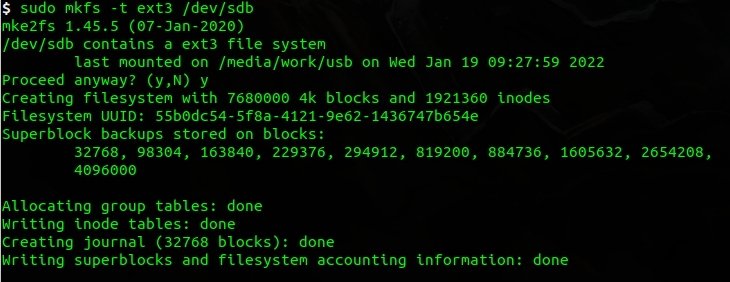
\includegraphics[width=12cm,keepaspectratio=true]{pictures/createfs.png}
	\caption{
		Erstellen eines EXT3 Dateisystems auf einem USB Stick
	}
	\label{fig:createfs}
\end{figure}

Im Abbildung \ref{fig:createfs} ist zu sehen wie das Dateisystem auf dem USB Stick unter "/dev/sdc" erstellt wird. Es werden 7680000 4KB Blöcke mit 1921360 Inodes erstellt (32GB). Für das Dateisystem wird eine \ac{uuid} generiert, ein Journal erstellt, sowie die Blöcke der Superblock-Backups ausgegeben.


\subsubsection{Erstellen von Dateien}

Folgendes Listing erzeugt eine Datei:

\begin{lstlisting}[language=bash]
# Asumming the fs is mounted on /media/usb
cd /media/usb
touch mydocument.txt
echo "Hallo welt." > mydocument.txt
\end{lstlisting} 

Mit Hilfe des Kommandos \textit{ls -li} können wir uns die Inode-ID ausgeben lassen um diese dann mit Hilfe des SleuthKit (\cite{Sleuthkit.07.01.2022}) Kommandos \textit{icat} näher zu betrachten.

\begin{figure}[H]
	\centering
	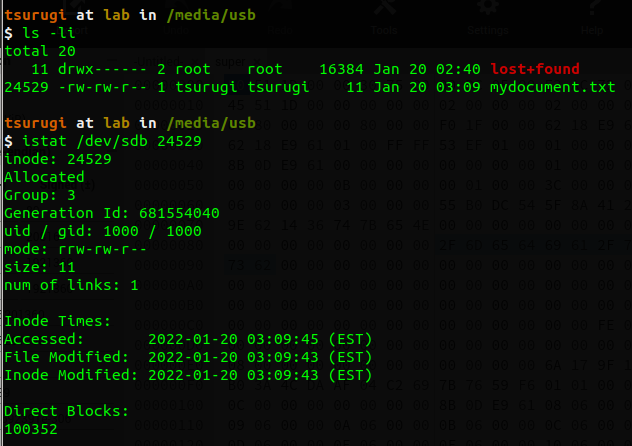
\includegraphics[width=12cm,keepaspectratio=true]{pictures/inode-stats.png}
	\caption{
		Informationen einer Inode
	}
	\label{fig:inodestats}
\end{figure}

Wir sehen in Abbildung \ref{fig:inodestats}, dass unsere zuvor erstellte Datei \textit{mydocument.txt} zur Inode 24529 gehört. Sie befindet sich in Blockgruppe 3, hat eine Größe von 11 Bytes (Inhalt: \textit{Hallo welt.}) und der Inhalt der Datei befindet sich in Block Nummer 100352.

Mit Hilfe von \textit{dd} wollen wir uns nun den Inhalt des Blocks 100352 ansehen, um zu verifizieren ob dort auch die Daten unerer Datei liegen:

\begin{figure}[H]
	\centering
	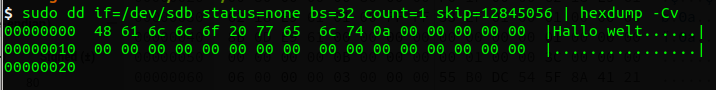
\includegraphics[width=12cm,keepaspectratio=true]{pictures/getfilecontent.png}
	\caption{
		Datei-Inhalt eines Blocks mit dd auslesen
	}
	\label{fig:getfilecontent}
\end{figure}

Da jeder Block in unserem Dateisystem 4096 Bytes groß ist, beginnt der Inhalt dieser Datei an Byteoffset 411041792 (Blocknummer x Blockgröße). Wir kopieren mit \textit{dd} immer 32 Byte, müssen daher mit Hilfe des \textit{skip}-Arguments angeben, ab wann wir mit dem Kopieren starten wollen (411041792/32 = 12845056). Und siehe da, der Inhalt der Datei wird korrekt ausgegeben!

Interessant ist, dass bei erneutem Schreiben in die Datei ein neuer Block verwendet wird, der alte immer noch die Daten des vorherigen Schreibvorgags enthält (Inode bleibt die Selbe):

TODO stackoverflow? sonst weglassen.

Das liegt daran, dass TODO!


TODO: edit und dann anderer Block??? WARUM NEUER BLOCK WENN ICH ECHO MACH!?!?!?!??!?!?!?!?!


\subsubsection{Löschen von Dateien}

Wir löschen die Datei mit folgemdem Kommando:

\begin{lstlisting}[language=bash]
rm -rf mydocument.txt
\end{lstlisting} 

Wir wissen noch die Inode ID 24529. Abbildung \ref{fig:istatafterdelete} zeigt die Analyse dieser Inode mittels \textit{istat} nach dem Löschen der Datei:

\begin{figure}[H]
	\centering
	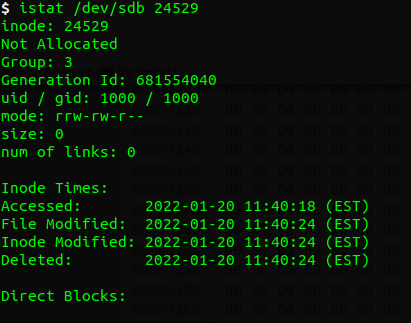
\includegraphics[width=12cm,keepaspectratio=true]{pictures/istatafterdelete.png}
	\caption{
		Datei-Inhalt eines Blocks mit dd auslesen
	}
	\label{fig:istatafterdelete}
\end{figure}

Die Inode ist nun nicht mehr allokiert (\textit{Not Allocated}), die Dateigröße beträgt nun 0 Byte und die Referenz zum Inhaltsblock wurde entfernt. Außerdem kam ein \textit{Deleted}-Datensatz hinzu. Dennoch können wir immer noch die Daten der vorherigen Blocknummer auslesen und bekommen den Inhalt der Datei. Es wird also nicht der Inhalt gelöscht, sondern nur die Referenz in der Inode gelöscht, sowie der Speicherplatz freigegeben.

\newpage

\section{Forensische Analyse des EXT3 Dateisystems}

a) Welche forensischen Konzepte existieren für die Auswertung eines EXT3 Dateisystems? 

TODO: ZUERST sleuthkit Vorstellung


sudo fsstat -o 0 /dev/sdb
FILE SYSTEM INFORMATION
--------------------------------------------
File System Type: Ext3
usw... CHECK DAS GENAU!


b) Welche Ansätze unter EXT3 gibt es, um eine gelöschte Datei wiederherzustellen?

vorher ggf mal ls -li und inode number merken!
dann rm -rf hier zeigen

UND dann SLEUTHKIT
Rekursives Anzeigen aller Dateien, inklusive gelöschter Dateien:
sudo fls -o 0 -r /dev/sdb
...
r/r * 24530:	Bildschirmfoto vom 2022-01-07 11-59-24.png

Dann Wiederherstellen der Datei mit inode 24530 mittels icat:
sudo icat -o 0 /dev/sdb 24530 > image.jpg


TODO: THIS WORKED!!!!!!!! auch mit rm -rf! MEHR EXPERIMENTE. WIE FUNZT DAS?
irgendwie mit dem journal. read man!
sudo ext4magic /dev/sdc -M




TODO: autopsy vorstellung und BEISPIEL!!!!!!!!!!!!!!!!!!!!!!!????????????

TODO recover on linux:\\
	https://possiblelossofprecision.net/?p=1216\\
	weitere tools linux: foremost, dff? ...\\
		-> https://www.cgsecurity.org/wiki/PhotoRec
	sudo ext4magic /dev/sdc -M

TODO:
READ this: https://en.wikipedia.org/wiki/Ext3




\subsection{Praktisches Beispiel}

1. Files erstellen und dann löschen (1mal mit papierkorb 1mal mit rm -rf - ggf auch ganzes DIR!)
2. Forensische Arbeitskopie erstellen:

\begin{lstlisting}
$ sudo dd if=/dev/sdc of=usb.dd bs=512 conv=noerror,sync status=progress
\end{lstlisting}

TODO beispiel:

Datei erstellen, löschen ist ja bereits in TEIL1 passiert! darauf verweisen, daran werde ich nun weiterarbeiten hier!

ERSTMAL ARBEITSKOPIE!!! ganzen prozess erklären (siehe forensics BOOK -> why, how etc...)
schön mit screenshots und code ausschnitten!

TODO: file listing node.js script zum auslesen von Datenblöcken ans Ende des Docs!!!!!!!!!!!!!!